\documentclass{beamer}
\usetheme{CambridgeUS}

\usepackage{amssymb, amscd,stmaryrd,setspace,hyperref,color}

\input xy
\xyoption{all} \xyoption{poly} \xyoption{knot}\xyoption{curve}


\newcommand{\longnote}[2][4.9in]{\fcolorbox{black}{yellow}{\parbox{#1}{\color{black} #2}}}
\newcommand{\shortnote}[1]{\fcolorbox{black}{yellow}{\color{black} #1}}
\newcommand{\start}[1]{\shortnote{Start here: #1.}}
\newcommand{\q}[1]{\begin{question}#1\end{question}}
\newcommand{\g}[1]{\begin{guess}#1\end{guess}}
\newcommand{\hsps}[1]{{\hspace{2mm} #1\hspace{2mm}}}

\def\mcB{\mathcal{B}}
\newcommand{\mcC}{\mathcal{C}}
\newcommand{\mcD}{\mathcal{D}}
\def\mcE{\mathcal{E}}
\newcommand{\mcG}{\mathcal{G}}
\def\mcS{\mathcal{S}}
\def\mcT{\mathcal{T}}
\def\mcX{\mathcal{X}}
\def\mcY{\mathcal{Y}}
\def\RR{{\mathbb R}}
\newcommand{\Ob}{{\bf Ob}}
\newcommand{\Arr}{{\bf Arr}}
\def\Path{{\bf Path}}
\newcommand{\Fun}{{\bf Fun}}
\newcommand{\taking}{\colon}
\newcommand{\too}{\rightarrow}
\newcommand{\toooo}{\longrightarrow}
\newcommand{\To}{\xrightarrow}
\newcommand{\Too}[1]{\To{\hsps{#1}}}
\newcommand{\tto}{\rightrightarrows}
\def\from{\leftarrow}
\newcommand{\From}{\xleftarrow}
\newcommand{\id}{\textnormal{id}}
\newcommand{\im}{\textnormal{im}}
\newcommand{\Sets}{{\bf Set}}
\def\Top{{\bf Top}}
\newcommand{\Set}{{\bf Set}}
\newcommand{\set}{{\text \textendash}{\bf Set}}
\newcommand{\Cat}{{\bf Cat}}
\newcommand{\Strings}{{\bf Strings}}
\newcommand{\NN}{{\mathbb N}}
\newcommand{\cross}{\times}
\newcommand{\iso}{\cong}
\newcommand{\sss}{\subset}
\newcommand{\tn}[1]{\textnormal{#1}}
\newcommand{\ul}[1]{\underline{#1}}
\newcommand{\ol}[1]{\overline{#1}}
\newcommand{\hsp}{\hspace{.2in}}
\newcommand{\comment}[1]{}
\newcommand{\bD}{{\bf \Delta}}
\def\Type{{\bf Type}}
\def\CPO{{\bf CPO}}
\newcommand{\obox}[3]{\stackrel{#1}{\fbox{\parbox{#2}{#3}}}}
\newcommand{\labox}[2]{\obox{#1}{1.6in}{#2}}
\newcommand{\mebox}[2]{\obox{#1}{1in}{#2}}
\newcommand{\smbox}[2]{\stackrel{#1}{\fbox{#2}}}
\newcommand{\LA}[2]{\ar[#1]^-{\tn {#2}}}
\newcommand{\LAL}[2]{\ar[#1]_-{\tn {#2}}}

\newcommand{\LMO}[1]{\bullet^{#1}}
\newcommand{\LTO}[1]{\bullet^{\tn{#1}}}


\newcommand{\fst}[2]{\subsection{#1}\frame{\frametitle{#1} #2}}
\newcommand{\ft}[2]{\frame{\frametitle{#1} #2}}

\def\sub{\begin{itemize}\item}
\def\next{\item}
\def\endsub{\end{itemize}}

\newcommand{\mainCatSmall}[1]{%  \mainCat{<Name>}
	\stackrel{#1}{
		\parbox{1.1in}{\tiny\fbox{\parbox{1.1in}{\tiny\underline{$m;d \simeq d$}\hsp  \underline{$s;d \simeq\id_D$\normalsize}\\\\
			\xymatrix@=4pt{&\LMO{E}\ar@<.5ex>[rrr]^d\ar@(l,u)[]^m\ar[ddl]_f\ar[ddr]^l&&&\LMO{D}\ar@<.5ex>[lll]^s\ar[dd]^n\\\\				\LMO{S}&&\LMO{S}&~&\LMO{S}}
		}}}
	}
}

\newcommand{\mainCatLarge}[1]{
	\stackrel{#1}{
		\parbox{2.3in}{\tiny\fbox{\parbox{2.3in}{\underline{Mgr;Dpt$ \simeq$ Dpt}\hsp  \underline{Secr;Dpt$ \simeq\id_{\tn{Department}}$}\\\\
			\xymatrix@=4pt{&\LTO{Employee}\ar@<.5ex>[rrrrr]^{\tn{Dpt}}\ar@(l,u)[]^{\tn{Mgr}}\ar[dddl]_{\tn{First}}\ar[dddr]^{\tn{Last}}&&&&&\LTO{Department}\ar@<.5ex>[lllll]^{\tn{Secr}}\ar[ddd]^{\tn{Name}}\\\\\\\LTO{String}&&\LTO{String}&~&~&~&\LTO{String}
			}
		}}}
	}
}


%%%%%%%%%%%%%%%%%%


\begin{document}

\title{Categorical databases}

\author{David I. Spivak}

\date{Presented on 2012/01/13}

\institute[MIT]{
  \url{dspivak@math.mit.edu}\\
  Mathematics Department\\
  Massachusetts Institute of Technology \\

}


\begin{frame}\titlepage \end{frame}

\section{Introduction}

\fst{Purpose of the talk}{

\large There is an fundamental connection between databases and categories.\normalsize\vspace{.2in}
	\sub Category theory can simplify how we think about and use databases.
	\next We can clearly see all the working parts and how they fit together.
	\next Powerful theorems can be brought to bear on classical DB problems.
	\endsub
}	

\fst{The pros and cons of relational databases}{
	\sub Relational databases are reliable, scalable, and popular.
	\next They are provably reliable to the extent that they strictly adhere to the underlying mathematics.
	\next Make a distinction between 
		\sub the system you know and love, {\em vs.}
		\next the relational model, as a mathematical foundation for this system.
		\endsub 
	\endsub}

\ft{You're not really using the relational model.}{
	\sub Current implementations have departed from the strict relational formalism:
		\sub Tables may not be relational (duplicates, e.g from a query). 
		\next Nulls (and labeled nulls) are commonly used.
		\endsub
	\next The theory of relations (150 years old) is not adequate to mathematically describe modern DBMS. 
	\next The relational model does not offer guidance for schema mappings and data migration.
	\next Databases have been intuitively moving toward what's best described with a more modern mathematical foundation.
	\endsub 

}

\ft{Category theory gives better description}{
	\sub Category theory (CT) does a better job of describing what's already being done in DBMS.
		\sub Puts functional dependencies and foreign keys front and center.
		\next Allows non-relational tables (e.g. duplicates in a query).
		\next Labeled nulls and semi-structured data fit in neatly.
		\endsub
	\next All columns of a table are the same type of thing. It's simpler.
	\next CT offers guidance for schema mapping and data migration.
	\next It offers the opportunity to deeply integrate programming and data.
	\next Theorems within category theory, and links to other branches of math (e.g. topology), can be used in databases.
	\endsub
}

\fst{What is category theory?}{
	\sub Since its invention in the early 1940s, category theory has revolutionized math.
	\next It's like set theory and logic, except less floppy, more principles-based.
	\next Category theory has been proposed as a new foundation for mathematics (to replace set theory).
	\next It was invented to build bridges between disparate branches of math by distilling the essence of mathematical structure.
	\endsub
}

\ft{Branching out}{
	\sub Category theory naturally fosters connections between disparate fields.
	\next It has branched out of math and into physics, linguistics, and materials science.
	\next It has had much success in the theory of programming languages.
	\next The pure category-theoretic concept of {\em monads} has vastly extended the reach of functional programming.
	\next Can category theory improve how we think about databases?
	\endsub

}

\subsection{The basic idea}

\ft{Schemas are categories, categories are schemas}{
	\sub The connection between databases and categories is simple and strong.
	\next Reason: categories and database schemas do the same thing.
		\sub A schema gives a framework for modeling a situation;
			\sub Tables
			\next Attributes
			\endsub
		\next This is precisely what a category does.
			\sub Objects
			\next Arrows.
			\endsub
		\next They both model how entities within a given context interact.
		\endsub
	\next Schema = Category.
	\next In this talk, I'll explain these ideas and some consequences.
	\endsub
}

%\fst{What this viewpoint brings to databases}{
%	\sub Conceptual clarity,
%	\next Easy integration with relational model,
%	\next Ability to define ``functorial" data migration and schema evolution,
%	\next Good understanding of views, queries, and constraints,
%	\next Integration with PL theory.
%	\endsub	
%}
%
%\ft{The theory extends the reach of relational}{
%	\sub The following occur naturally in the category-theoretic, but not the relational model.
%		\sub Labelled nulls,
%		\next Query results that are not relational,
%		\next Row ``numbers",
%		\next Relaxing into RDF and semi-structured data.
%		\endsub
%	\next The first three are found in most {\em implementations} of relational databases, but are not in the relational model. 
%	\endsub
%}
%

\fst{Plan of the talk}{
	\sub Lay out the basic idea of categories and that of databases, and show the tight connection between them.
	\next Discuss schema evolution and data migration.
	\next Develop a connection to programming language theory.
	\next Understand RDF in these terms.
	\endsub
}


\section{``Databases are categories"}

\subsection{First some math}

\ft{What is a category?}{
	\sub Idea: A category models entities of a certain sort \\and the relationships between them.$$\mcC:=\parbox{2in}{\fbox{\xymatrix{\bullet^A\ar[r]^f&\bullet^B\ar@/_1pc/[r]_h\ar@/^1pc/[r]^g&\bullet^C\\\bullet^D\ar@(l,u)[]^i\ar@/^1pc/[r]^j&\bullet^E\ar@/^1pc/[l]^k}}}$$ 
	\next Think of it like a graph: the nodes are entities and the arrows are relationships.
	\next Some paths can be declared equivalent to others
		\sub Example: declare that $j;k \simeq i;i;i$ and $f;g \simeq f;h$.
		\endsub
\endsub

}

\ft{Example}{
	\sub How could one interpret this kind of abstraction? $$\mcC:=\parbox{2.2in}{\fbox{\parbox{2.2in}{\parbox{2in}{\tiny self email is an email from a person =\\self email is an email to a person\normalsize}\\\\\xymatrix{\LTO{Self-email}\ar[r]^{\tn{is an}}&\LTO{Email}\ar@/_1pc/[r]_{\tn{to a}}\ar@/^1pc/[r]^{\tn{from a}}&\LTO{Person}}}}}$$
	\next Such ``business rules" can be encoded into the category.
	\endsub

}

\ft{What is the essence of structure?}{
	\sub If mathematics is the art of getting organized, what organizes math?
	\next After thousands of years, people realized that there were some essential features in common throughout much of math.
	\next These are objects, arrows, paths, and path equivalence.
	\next Or: things, tasks, processes, and ``sameness of outcome".
	\next Or: primary keys, foreign keys, paths of FKs, and path equations.
	\next Let's give the definition.
	\endsub
}

\ft{Definition of a category I: Constituents}{

A {\em category} $\mcC$ consists of the following constituents:
\begin{enumerate}
\item A set $\Ob(\mcC)$, called {\em the set of objects of $\mcC$}. 
	\sub (These will be tables.)
	\next Objects $x\in\Ob(\mcC)$ is often written as $\bullet^x$.
	\endsub
\item A set $\Arr(\mcC)$, called {\em the set of arrows of $\mcC$}, and two functions $$src,tgt\taking\Arr(\mcC)\to\Ob(\mcC),$$ assigning to each arrow its {\em source} and its {\em target} object, respectively.
	\sub (Arrows will be foreign keys from ``source" table to ``target" table.)
	\next An arrow $f\in\Arr(\mcC)$ is often written $\LMO{x}\Too{f}\LMO{y}$, where $x=src(f), y=tgt(f)$.
	\next We define a {\em path in $\mcC$} to be a finite ``head-to-tail" sequence of arrows in $\mcC$, e.g. $\LMO{x}\Too{f}\LMO{y}\Too{g}\LMO{z}$.
	\endsub
\item An notion of equivalence for paths, denoted $\simeq$.
\end{enumerate} 

}

\ft{Definition of a category II: Rules}{

These constituents must satisfy the following requirements:
	\begin{enumerate}
	\item If $p \simeq q$ are equivalent paths then the sources agree: $src(p)=src(q).$
	\item If $p \simeq q$ are equivalent paths then the targets agree: $tgt(p)=tgt(q).$
	\item Suppose we have two paths (of any lengths) $b\to c$: $$\xymatrix@=13pt{&\bullet\ar[r]&\cdots\ar[r]&\bullet\ar[dr]\\\LMO{b}\ar[ur]\ar[dr]\ar@{-->}@/^1.5pc/[rrrr]_p\ar@{-->}@/_1.5pc/[rrrr]^q&&&&\LMO{c}\\&\bullet\ar[r]&\cdots\ar[r]&\bullet\ar[ur]}$$ If $p \simeq q$ then for any extensions$$\xymatrix{\LMO{a}\ar[r]^m&\LMO{b}\ar@{}[rr]|{\simeq}\ar@{-->}@/^1pc/[rr]^p\ar@{-->}@/_1pc/[rr]_q&&\LMO{c}} \hsp\tn{or}\hsp\xymatrix{\LMO{b}\ar@{-->}@/^1pc/[rr]^p\ar@{}[rr]|{\simeq}\ar@{-->}@/_1pc/[rr]_q&&\LMO{c}\ar[r]^n&\LMO{d}}$$\hspace{.5in} $m;p \simeq m;q$\hspace{.75in} and\hspace{.75in} $p;n \simeq q;n$.
	\end{enumerate}
}

\fst{What does equivalence of paths mean?}{
	\sub Arrows represent foreign keys.
	\next A path $p\taking\LMO{a}\to\LMO{b}$ represents ``following foreign keys" from table $a$ to table $b$.
	\next Following a path $p$, we can take any record in table $a$ and return a record in table $b$.
	\next We declare two paths $p,q\taking \LMO{a}\to\LMO{b}$ equivalent if they should return the same record in $b$ for any record in $a$.  	
	\next In typical DB practices, equivalent paths are avoided by cutting one of the paths. 
		\sub This is considered good design.
		\next However, it often causes pain in ones neck. 
		\next Category theory has this concept built in.
		\endsub
	\endsub
}

\ft{The power of path equivalences}{
	\sub Ever wanted two directory paths to contain the same file?
	\next Example: this ``Beamer" presentation belongs in my math talks folder and in my J\&J consulting folder.
	\next My file system does not allow that, because without path equivalences, it is dangerous.
	\next With commutative diagrams we can declare two paths equivalent: $$\xymatrix{\LTO{J\&J talks}\ar[d]\ar[r]&\LTO{J\&J Consulting stuff}\ar@{}[d]|(.4){\checkmark}\ar[r]&\LTO{Consulting stuff}\ar[d]\\\LTO{Math talks}\ar[r]&\LTO{Math stuff}\ar[r]&\LTO{All files (root)}}$$
	\endsub
}


\subsection{Examples of categories}

\ft{The category of Sets}{
	\begin{center}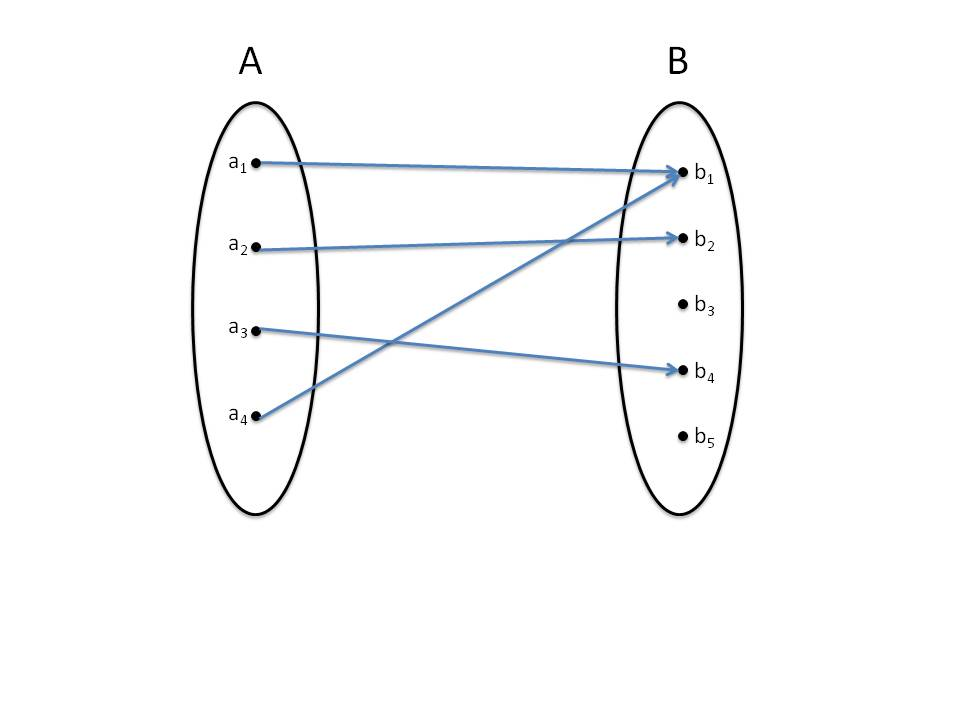
\includegraphics[height=5cm]{SetMap}\end{center}\vspace{-.6in}
	\sub Above we see two sets and a function between them. We would denote this categorically by $\LMO{A}\Too{f}\LMO{B}$
		\sub The objects of $\Set$ represent sets.
		\next The arrows in $\Set$ represent functions.
		\next A path represents a sequence of composable functions.
		\next Two paths are equivalent if their compositions are the same.
		\endsub
	\next Note that $b_3$ and $b_5$ have been inserted, and $a_1$ and $a_4$ have been merged.
	\endsub
}

\ft{A totally different category: an ordered set}{
	\sub A ordered set is a set $S$ together with a notion of $\leq$, satisfying
		\sub $a\leq a$ for all $a\in S$, and
		\next if $a\leq b$ and $b\leq c$, then $a\leq c$.
		\endsub
	\next Given some ordered set $S$, we can build a corresponding category $\mcS$: 
		\sub $\Ob(\mcS)=S$,
		\next One arrow $a\to b$ if $a\leq b$
		\next No arrows $a\to b$ if $a\not\leq b$.
		\next All pairs of paths (having same source and target) are equivalent.
		\endsub
	\next ``Hasse diagram": $$\xymatrix@=8pt{\LMO{a}\ar[drr]&&&&\LMO{b}\\&&\LMO{c}\ar[urr]\ar[drr]\\\LMO{d}\ar[urr]\ar[drr]&&&&\LMO{e}&&\LMO{f}\\&&\LMO{g}\ar[urr]}$$
	\next Think ``permissions": $a\leq c$ means $a$ has fewer accessors than $b$. 
	\endsub
}
	
\ft{Functors: mappings between categories}{

	\sub One way to think of a category is as a directed graph, where certain paths have been declared equivalent.
	\next A functor is a graph mapping that is required to respect equivalence of paths.\vspace{.1in}
	\next {\bf Definition}: A functor $F\taking\mcC\to\mcD$ consists of 
		\sub a function $\Ob(\mcC)\to\Ob(\mcD)$ and
		\next a function $\Arr(\mcC)\to\Path(\mcD)$, 
		\endsub
such that $F$
		\sub respects sources and targets,
		\next respects equivalences of paths.
		\endsub\vspace{.1in}
	\endsub
}


\fst{Functors to $\Set$}{

	\sub A category $\mcC$ is a system of objects and arrows, and an equivalence relation on its paths.
	\next A functor $\mcC\too\mcD$ is a mapping that preserves these structures.
	\next $\Set$ is the category whose objects are sets, whose arrows are functions, and where paths are equivalent if they compose to the same function.
	\next If $\mcC$ is the category on the left below, then a functor $I\taking\mcC\too\Set$ might look like this: $$\mcC:=\parbox{.9in}{\fbox{\xymatrix{A\ar[r]^f\ar[d]_g&B\\C}}};\hspace{.2in} I:=\parbox{2.7in}{\fbox{\xymatrix{\fbox{$\bullet_{a_1}\bullet_{a_2}\bullet_{a_3}$}\ar[rr]^{\parbox{.35in}{\tiny\begin{spacing}{1}$a_1\mapsto b_1\\a_2\mapsto b_1\\a_3\mapsto b_2$\end{spacing}\normalsize}}\ar[d]&&\fbox{$\bullet_{b_1}\bullet_{b_2}$}\\\fbox{$\bullet_{c_1}$}}}}$$
	
	\endsub

}


%\ft{Functors between two ordered sets}{
%	\sub Suppose $\mcS$ and $\mcT$ are categorical representations of ordered sets $S$ and $T$.
%	\next What is the meaning of a functor $F\taking\mcS\to\mcT$?
%	\next Answer: 
%		\sub a function $F$ from the elements of $S$ to the elements of $T$, such that
%		\next if $s\leq s'$ then $F(s)\leq F(s')$.
%		\endsub
%	\next Here, functors provide a very reasonable notion of mapping.
%	\next Functors are always reasonable because they preserve everything you cared enough about to put into the structure of your category.
%	\endsub
%}
%
%
%\ft{Functors from an ordered set to $\Set$}{
%	\sub Let $\mcS$ be the categorical representation of an ordered set $S$.
%	\next What is the meaning of a functor $A\taking\mcS\to\Set$?
%	\next Answer:
%		\sub For every element $s\in S$ we have a set $A(s)$ of ``accessors", and
%		\next given $s\leq s'$ we have a function $A(s)\to A(s')$.
%		\endsub 
%	\next (We may want to instead look at functors $\mcS\to{\bf Inj}$, i.e. only allow injective functions..)
%	\next Such functors on $\mcS$ capture permissions.
%	\endsub
%}
	 
%\ft{Foreign keys simply give functions}{
%	\begin{align*}\begin{tabular}{| c || c | c |}\hline\multicolumn{3}{| c |}{Member}\\\hline {\bf Id}&{\bf is type}&{\bf is in}\\\hline $a_1$&$b_1$&$c_1$\\\hline $a_2$ & $b_1$&$ c_1$\\\hline $a_3$&$b_2$&$c_1$\\\hline\end{tabular}\hsp\begin{tabular}{| c ||}\hline \multicolumn{1}{| c |}{Element}\\\hline{\bf Id}\\\hline $b_1$\\\hline $b_2$\\\hline\end{tabular}\hsp\begin{tabular}{| c ||}\hline \multicolumn{1}{| c |}{Collection}\\\hline{\bf Id}\\\hline $c_1$\\\hline\end{tabular}\end{align*}
%	Each foreign key column represents a function.
%	$$\parbox{.9in}{\fbox{\xymatrix{\LTO{Member}\LA{r}{is type}\LAL{d}{is in}&\LTO{Element}\\\LTO{Collection}}}}$$
%
%}	



\subsection{How we're thinking of databases}

\fst{What is a database?}{

	\sub A database consists of a bunch of tables and relationships between them.
	\next The rows of a table are called ``records" or ``tuples."
	\next The columns are called ``attributes."
	\next An attribute may be ``pure data" or may be a ``key."
		\sub A table may have ``foreign key columns" that link it to other tables.
		\next A foreign key of table $A$ links into the primary key of table $B$.
		\endsub
	\next A schema may have ``business rules."
	\endsub

}

\fst{Foreign Keys and business rules}{

	\sub Example:\tiny \begin{align*}&\begin{tabular}{| l || l | l | l | l |}\hline\multicolumn{5}{| c |}{Employee}\\\hline {\bf Id}&{\bf First}&{\bf Last}&{\bf Mgr}&{\bf Dpt}\\\hline 101&David&Hilbert&103&q10\\\hline 102&Bertrand&Russell&102&x02\\\hline 103&Alan&Turing&103&q10\\\hline\end{tabular}&\begin{tabular}{| l || l | l |}\hline\multicolumn{3}{| c |}{Department}\\\hline {\bf Id}&{\bf Name}&{\bf Secr}\\\hline q10&Sales&101\\\hline x02&Production&102\\\hline\end{tabular}\end{align*}\normalsize
	\next Note the Id (primary key) columns and the foreign key columns.
		\sub Id column could just be internal ``row numbers" or could be typed.
		\next ``Row numbers" (i.e. pointers) are not part of the relational model but they are naturally part of the categorical model.
		\endsub
	\next Perhaps we should enforce certain integrity constraints (business rules):
		\sub The manager of an employee $E$ must be in the same department as $E$,
		\next The secretary of a department $D$ must be in $D$.
		\endsub
	\endsub

}

\ft{Data columns as foreign keys}{

	\sub Theoretically we can consider a data-type as a 1-column table.
	\next Examples: \tiny$$\begin{tabular}{| l |}\hline\multicolumn{1}{| c |}{\bf String}\\\hline a\\\hline b\\\hline \vdots\\\hline z\\\hline aa\\\hline ab\\\hline\vdots\\\hline\end{tabular}\hsp\hsp\hsp\begin{tabular}{| l |}\hline\multicolumn{1}{| c |}{\bf Integer}\\\hline 0\\\hline 1\\\hline \vdots\\\hline 9\\\hline 10\\\hline 11\\\hline\vdots\\\hline\end{tabular}$$\normalsize
	\next So even data columns can be considered as foreign keys (to respective 1-column tables).
	\next Conclusion: each column in a table is a key -- one primary,\\ the rest foreign.
	\endsub
}

\ft{Example again}{

\tiny \begin{align*}&\begin{tabular}{| l || l | l | l | l |}\hline\multicolumn{5}{| c |}{Employee}\\\hline {\bf Id}&{\bf First}&{\bf Last}&{\bf Mgr}&{\bf Dpt}\\\hline 101&David&Hilbert&103&q10\\\hline 102&Bertrand&Russell&102&x02\\\hline 103&Alan&Turing&103&q10\\\hline\end{tabular}&\begin{tabular}{| l || l | l |}\hline\multicolumn{3}{| c |}{Department}\\\hline {\bf Id}&{\bf Name}&{\bf Secr}\\\hline q10&Sales&101\\\hline x02&Production&102\\\hline\end{tabular}&&\begin{tabular}{| l |}\hline\multicolumn{1}{| c |}{ String}\\\hline {\bf Id}\\\hline a\\\hline b\\\hline \vdots\\\hline z\\\hline aa\\\hline ab\\\hline\vdots\\\hline\end{tabular}&\end{align*}


\tiny$$\mcC:=\mainCatLarge{}$$\normalsize

}




\fst{Database schema as a category}{

	\sub A database schema is a system of tables linked by foreign keys.
	\next This is just a category! 
		\tiny$$\mcC:=\mainCatLarge{}$$\normalsize
		\sub Each object $x$ in $\mcC$ is a table (Employee, Departments, String);
		\next each arrow $x\to y$ is a column of table $x$.
		\endsub
	\next Id column of a table corresponds to the trivial path on that object.
	\next Declaring business rules (e.g.  Mgr;Dpt$ \simeq$ Dpt) is declaring the path equivalence.
	\endsub
}

\fst{Schema=Category, Instance=Set-valued functor}{

\sub Let $\mcC$ be the following category \tiny$$\mcC:=\mainCatLarge{}$$\normalsize

	\next A functor $I\taking\mcC\to\Sets$ consists of 
		\sub A set for each object of $\mcC$ and
		\next a function for each arrow of $\mcC$, such that
		\next the declared equations hold.
		\endsub
	\next In other words, $I$ fills the schema with compatible data.
	\next Categorical databases could also be called {\em functional databases}.  
	\endsub

}

\ft{Data as a set-valued functor}{

\tiny\begin{align*}&\mcC:=&I\taking\mcC\too\Sets\\&\fbox{\parbox{1.7in}{\underline{$m;d \simeq d$}\hsp  \underline{$s;d \simeq \id_D$}\\\\\xymatrix{\bullet_{\tn{Emp}}\ar@<.5ex>[rr]^d\ar@(l,u)[]^m\ar[d]_f\ar[dr]^l&&\bullet_{\tn{Dpt}}\ar@<.5ex>[ll]^s\ar[d]^n\\\LMO{Str}&\LMO{Str}&\LMO{Str}}}}&\fbox{\parbox{1.8in}{\xymatrix{\fbox{101,102,103}\ar@<.5ex>[rr]^d\ar@(l,u)[]^m\ar[d]_f\ar[dr]^l&&\fbox{q10,x02}\ar@<.5ex>[ll]^s\ar[d]^n\\\fbox{a,b,\ldots}&\fbox{a,b,\ldots}&\fbox{a,b,\ldots}}}}\end{align*}.\normalsize


	\sub A category $\mcC$ is a schema.  An object $x\in\Ob(\mcC)$ is a table.
	\next A functor $I\taking\mcC\too\Sets$ fills the tables with compatible data.
	\next For each table $x$, the set $I(x)$ is its set of rows.
	\next The path equivalences in $\mcC$ are enforced by $I$ as business rules.
	\endsub
}

\ft{Summary}{
	\sub The connection between categories and databases is simple.
	\next A schema is a custom category.
	\next Functors $I\taking\mcC\to\Set$ are instances.
	\next What about functors $F\taking\mcC\to\mcD$ between schemas?
	\endsub
}



\section{Functorial schema mapping and data migration}

\fst{Changes}{
	\sub We've discussed the situation as though static: a single schema and a single instance.
	\next Next we'll discuss changes.
	\next Changing the schema (schema mappings).
	\next Changing the data (updates).
	\endsub
}

\fst{Changes in schema}{
	\sub Suppose in our modeling of a given context, we evolve from schema $\mcC$ to schema $\mcD$.
	\next We should find a functorial connection between them.
	\next Over time we may have something like $$\mcC=\mcC_0\Too{F_0}\mcC_1\Too{F_1}\cdots\Too{F_n}\mcC_n=\mcD$$
	\next We want to be able to migrate data from $\mcC$ to $\mcD$ and vice versa.
	\next We want to be able to migrate queries against $\mcC$ to queries against $\mcD$ and vice versa.
	\next And we want this all to work as it ``should".
	\endsub
}


\ft{Composing functors}{
	\sub Suppose $F\taking \mcC\to\mcD$ and $G\taking\mcD\to\mcE$ are functors.
	\next What is their composition $\mcC\to\mcE$?
		\sub We have a way to take objects in $\mcC$ to objects in $\mcE$,
		\next Arrows in $\mcC$ turn into paths in $\mcD$ and arrows in $\mcD$ turn into paths in $\mcE$.
		\next We can concatenate these, thus taking arrows in $\mcC$ to paths in $\mcE$.
		\next Our rules ensure that the equivalences in $\mcC$ will be preserved in $\mcE$.
		\endsub
	\next Composing functors is going to make migrating data more straightforward.
	\endsub
}

\fst{Changes in data}{
	\sub Let $\mcC$ be a schema and let $I,J\taking\mcC\to\Set$ be two instances.
	\next A {\em natural transformation} $u\taking I\to J$ consists of the following:
		\sub For each object (table) $T\in\Ob(\mcC)$ we get a map of record sets $$u_T\taking I(T)\to J(T).$$
		\next For each arrow (foreign key) $f\taking T\to T'$, we get data consistency; formally, $$J(f)\circ u_T=u_{T'}\circ I(f).$$
		\endsub
	\next If $J$ is the result of an insert or merge (a {\em progressive update}) to $I$ then $$u\taking I\to J.$$
	\next Same thing if $I$ is the result of a delete or a split (a {\em regressive update}) to $J$.
	\endsub
}
			
\ft{The category of instances}{
	\sub Given a schema $\mcC$, the {\em category of instances} on $\mcC$ is denoted $\mcC\set$.
		\sub The objects of $\mcC\set$ are functors (instances) $I\taking\mcC\to\Set$.
		\next The arrows are natural transformations (progressive updates).
		\next The paths are sequences of progressive updates.
		\next Two paths are equivalent if they result in the same mapping.
		\endsub
	\next The category $\mcC\set$ is a topos; it has an internal language and logic supporting the {\em typed lambda calculus}.
	\next That means, it works well with the theory of programming languages.
	\endsub
}

\fst{Data migration}{
	\sub Let $\mcC$ and $\mcD$ be different schemas.
	\next We call a functor between them, $F\taking\mcC\to\mcD$, a {\em schema mapping}.
	\next Given such a mapping, we want to be able to canonically transfer instances on $\mcC$ to instances on $\mcD$ and vice versa.
	\next That means, given $F\taking\mcC\to\mcD$ we want functors $$\mcC\set\to\mcD\set$$ and $$\mcD\set\to\mcC\set.$$
	\endsub
}

\ft{What a functor $\mcC\set\to\mcD\set$ means.}{
A functor $\mcC\set\to\mcD\set$ means:
	\sub {\bf Objects:} To every instance on $\mcC$ we associate an instance on $\mcD$.
	\next {\bf Arrows:} For every progressive update on a $\mcC$-instance there is a corresponding progressive update on the associated $\mcD$-instance.
	\next {\bf Path equivalences:} If two different sequences of progressive updates on $\mcC$-instances result in the same mapping, then the same will hold of the corresponding sequences on $\mcD$-instances.
	\endsub  

}

\fst{The ``easy" migration functor, $\Delta$}{

	\sub Given a schema mapping (i.e. a functor) $$F\taking\mcC\too\mcD,$$ we can transform instances on $\mcD$ to instances on $\mcC$ as follows:$$\tn{\tiny Given $I\taking\mcD\to\Set$}\normalsize\hsp\hsp\xymatrix{\mcC\ar[r]^F\ar@/_1pc/[rr]_{F;I}&\mcD\ar[r]^-{I}&\Set}\hsp\hsp\tn{\tiny get $F;\!I\taking\mcC\to\Set$\normalsize}$$
	\next This process will preserve updates: given an update on $I$ on schema $\mcD$, it will spit out a corresponding update of $(F;I)$ on schema $\mcC$.
	\next Thus we have a functor $\Delta_F\taking\mcD\set\too\mcC\set$.
	\endsub

}

\ft{How $\Delta_F$ works}{
	\sub Consider the schema mapping \tiny$$\parbox{1.2in}{\begin{center}$\mcC:=$\end{center}\fbox{\parbox{1.1in}{\xymatrix@=15pt{&\LTO{DptName}\\\LTO{Emp}\ar[d]\ar[dr]\ar[r]\ar[ur]&\LTO{FrstNm}\\\LTO{SecLstNm}&\LTO{LstNm}}}}\vspace{.2in}}\Too{F}\mainCatLarge{\mcD:=}$$\normalsize
	\next We get $\Delta_F\taking\mcD\set\to\mcC\set$
	\next Given an instance on $\mcD$ we get one on $\mcC$.
	\next Given an update on $\mcD$ we get one on $\mcC$.
	\endsub
}

\ft{Compare the Informatica picture}{
\parbox{5in}{\tiny$$\stackrel{\mcC=}{\parbox{1.1in}{\fbox{\parbox{1.1in}{\xymatrix@=8pt{&\LTO{DptName}\\\LTO{Emp}\ar[d]\ar[dr]\ar[r]\ar[ur]&\LTO{FrstNm}\\\LTO{SecLstNm}&\LTO{LstNm}}}}}}\Too{F}\stackrel{\mcD=}{\parbox{1.1in}{\tiny\fbox{\xymatrix@=4pt{&\LTO{Emp}\ar@<.5ex>[rrr]^d\ar@(l,u)[]^m\ar[ddl]_f\ar[ddr]^l&&&\LTO{Dept}\ar@<.5ex>[lll]^s\ar[dd]^n\\\\\LTO{Str}&&\LTO{Str}&~&\LTO{Str}}}}}
$$\normalsize}\vspace{.2in}
\parbox{5in}{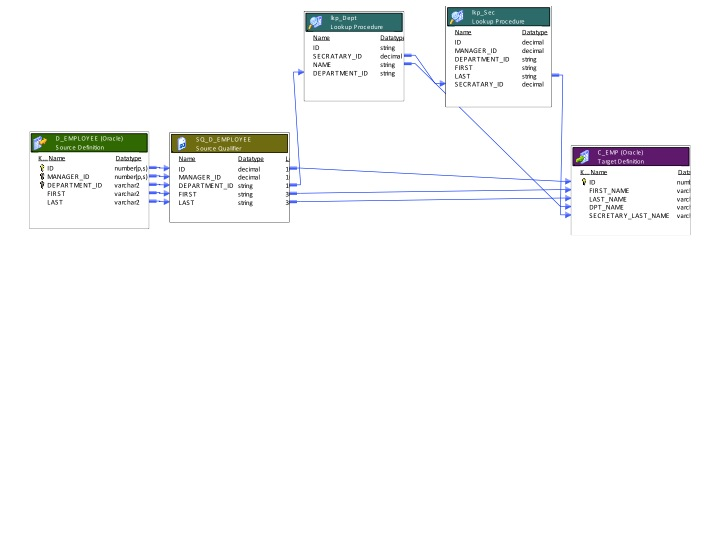
\includegraphics[height=8cm]{informatica}}
}

\ft{So many kinds of functors..}{
	\sub Functors in three different contexts.
		\sub We started with functors as instances, $I\taking\mcC\to\Set$.
		\next Then we introduced functors as schema mappings, $F\taking\mcC\to\mcD$.
		\next In the last slide we showed a functor on instance categories $$\Delta_F\taking\mcD\set\to\mcC\set.$$
		\endsub
	\next Recall the simple definition of functor we gave at the beginning: it holds in each case.
	\next Functors provide a powerful and reusable abstraction because of the simplicity of their definition.
	\endsub
}

\ft{Adjoints}{
	\sub 	Some functors $\mcX\to\mcY$ have a ``special partner" $\mcY\to \mcX$ called an {\em adjoint}.
	\next What it will mean to us is that we can always ``invert" a data migration $\mcD\set\to\mcC\set$ in two universal ways.
		\sub Roughly, our first inversion will be universal for progressive updates.
		\next Our second inversion will be universal for regressive updates.
		\endsub
	\next These migration functors will provide something like updatable views.
	\next The important thing is to note is that these aren't made up; they are ``canonical" or ``universal". They're part of the mathematics -- they come with the package.
	\endsub
}

\fst{The ``adjoint" migration functors, $\Sigma$ and $\Pi$}{
Given a schema mapping (i.e. a functor) $F\taking\mcC\too\mcD$, 
	\sub We have a functor $\Delta_F\taking\mcD\set\to\mcC\set$ given by composition.
	\next It has two adjoints:
		\sub a ``sum-oriented" adjoint $\Sigma_F\taking\mcC\set\to\mcD\set$, and
		\next a ``product-oriented" adjoint $\Pi_F\taking\mcC\set\to\mcD\set$.		
		\endsub
	\next Thus, given a schema mapping $F$, three functors emerge for the instance categories, $$\Delta_F,\Sigma_F, \tn{ and } \Pi_F$$ come with the package.
	\next Roughly, these correspond to project ($\Delta$), union ($\Sigma$), and join ($\Pi$).
	\next They allow one to move data back and forth between $\mcC$ and $\mcD$ in canonical ways.
	\endsub

}

\ft{The ``product-oriented" push-forward $\Pi_F$ makes joins}{
$$\stackrel{\mcC:=}{\parbox{2.25in}{\fbox{\xymatrix@=.1cm{&\bullet^{a_1}\ar[ddl]\ar[dd]\ar[ddr]\ar[rrr]&&&\bullet^{a_2}\ar[dd]\ar[rr]&&\bullet^{a_3}\ar[dd]\ar[ddr]\\\\\bullet^{b_1}&\bullet^{b_2}&\bullet^{b_3}&&\bullet^{c_1}&&\bullet^{d_1}&\bullet^{d_2}}}}}\Too{F}\stackrel{\mcD:=}{\parbox{2.1in}{\fbox{\xymatrix@=.1cm{&\bullet^a\ar[ddl]\ar[dd]\ar[ddr]\ar[ddrr]\ar[ddrrr]\ar[ddrrrr]\\\\\bullet^{b_1}&\bullet^{b_2}&\bullet^{b_3}&\bullet^{c_1}&\bullet^{d_1}&\bullet^{d_2}}}}}$$
	\sub We begin with three tables (with 3,1, and 2 data columns respectively) arranged in a detail to master hierarchy.
	\next Apply the ``product-oriented" push-forward $\Pi_F$ to join them into one table.
	\endsub
}

\ft{More joins using $\Pi_F$}{
%$$\fbox{\xymatrix{&\LTO{Salary}\\&\LTO{First}&\LTO{T2}\ar[lu]\ar[l]\ar[ld]\\\LTO{T1}\ar[ur]\ar[r]\ar[dr]&\LTO{Last}\\&\LTO{SSN}}}\stackrel{G}{\too}$$

$$\parbox{1.5in}{\fbox{\xymatrix@=10pt{&\LTO{SSN}\\&\LTO{First}\\\LTO{T1}\ar[uur]\ar[ur]\ar[dr]&&\LTO{T2}\ar[ul]\ar[dl]\ar[ddl]\\&\LTO{Last}\\&\LTO{Salary}}}}\Too{F}\parbox{1.2in}{\fbox{\xymatrix@=10pt{&\LTO{SSN}\\&\LTO{First}\\\LTO{U}\ar[uur]\ar[ur]\ar[dr]\ar[ddr]\\&\LTO{Last}\\&\LTO{Salary}}}}$$

}

\ft{The ``sum-oriented" push-forward $\Sigma_F$ makes unions}{
$$\stackrel{\mcC:=}{\parbox{1.5in}{\fbox{\xymatrix@=10pt{&\LTO{SSN}\\&\LTO{First}\\\LTO{T1}\ar[uur]\ar[ur]\ar[dr]&&\LTO{T2}\ar[ul]\ar[dl]\ar[ddl]\\&\LTO{Last}\\&\LTO{Salary}}}}}\Too{F}\stackrel{\mcD:=}{\parbox{1in}{\fbox{\xymatrix@=10pt{&\LTO{SSN}\\&\LTO{First}\\\LTO{U}\ar[uur]\ar[ur]\ar[dr]\ar[ddr]\\&\LTO{Last}\\&\LTO{Salary}}}}}$$

	\sub Given any instance $I\taking\mcC\to\Set$, get an instance $\Sigma_F(I)\taking\mcD\to\Set$.
	\next The rows in table $\LTO{U}$ will be the union of the rows in $\LTO{T1}$ and $\LTO{T2}$.
	\next It will automatically use labeled nulls for the unknown cells.
	\endsub
}


\fst{Views}{

	\sub These functors can be arbitrarily composed to create views.
	\next We can think of any series of functors $$\xymatrix{\mcC_1&\mcD_1\ar[l]_{F_1}\ar[r]^{G_1}&\mcE_1\ar[r]^{H_1}&\mcC_2&\mcD_2\ar[l]_{F_2}\ar[r]^{G_2}&\cdots\ar[r]^{H_n}&\mcC_n}$$ as a view.
	\next The view is the functor $$V:=\Sigma_{H_n}\circ\cdots\circ\Pi_{G_1}\circ\Delta_{F_1}\taking\mcC_1\set\to\mcC_n\set.$$
	\next We can export data from $\mcC_1$ into $\mcC_n$ through $V$.
	\next Note that $\mcC_n$ is a schema: not just one table, but possibly many, with foreign keys.
	\next It's no problem to create views that have foreign keys (unsupported in DBMS).
	\endsub
}


%\ft{Example of a view}{
%Here are some easy-to-understand schema mappings.
%\vspace{-.7in}\tiny$$\parbox{1.5in}{$\mcB$:=\\\fbox{\xymatrix@=3pt{&&\LTO{boy}\ar[ddll]\ar[ddrr]\\&&\LTO{man}\ar[dll]\ar[drr]\\\LTO{name}&&&&\LTO{address}\ar[dd]\\&&\LTO{woman}\ar[ull]\ar[urr]\\&&\LTO{girl}\ar[uurr]\ar[uull]&&\LTO{street}\ar[dd]\\\\&&&&\LTO{city}}}}\From{F}
%\parbox{1.4in}{$\mcC$:=\\\fbox{\xymatrix@=3pt{&&\LTO{boy}\ar[ddll]\ar[ddrr]\\&&\LTO{man}\ar[dll]\ar[drr]\\\LTO{name}&&&&\LTO{street}\\&&\LTO{woman}\ar[ull]\ar[urr]\\&&\LTO{girl}\ar[uurr]\ar[uull]}}}\To{G}
%\parbox{1.3in}{\vspace{1in}$\mcD$:=\\\fbox{\xymatrix@=1pt{&&\LTO{male}\ar[ddll]\ar[ddrr]\\\\\LTO{name}&&&&\LTO{street}\\\\&&\LTO{female}\ar[uurr]\ar[uull]}}\begin{center}$\downarrow H$\end{center}\hspace{-.15in}
%$\mcE$:=\fbox{\xymatrix@=1pt{&&\LTO{male}\ar[ddll]\ar[ddrr]\\\\\LTO{name}&&\LMO{Q}\ar[uu]\ar[dd]\ar@{}[rr]|(.4)*+{\checkmark}&&\LTO{street}\\\\&&\LTO{female}\ar[uurr]\ar[uull]}}}$$\normalsize
%
%	\sub We can formulate the view $V=\Pi_H\circ\Sigma_G\circ\Delta_F\taking\mcB\set\to\mcE\set.$
%	\next The view gives ``pairs of males and females living on the same street".
%	\endsub
%}

\frame{\frametitle{A simple ``SELECT" query using views}

SELECT title, isbn\\FROM book\\WHERE price $>100$\\

\tiny$$\parbox{1.7in}{$\mcC:=$\\\fbox{\xymatrix@=5pt{&&\LTO{book}\ar[rr]^{\tn{title}}\ar[rrdd]^{\tn{isbn}}\ar[dd]^{\tn{price}}&&\LTO{String}\\\\\LMO{\RR_{>100}}\ar[rr]&&\LMO{\RR}&&\LTO{isbn-num}}}}\To{F}\parbox{1.7in}{$\mcD:=$\\\fbox{\xymatrix@=5pt{\LMO{W}\ar[rr]\ar[dd]\ar@{}[ddrr]|{\checkmark}&&\LTO{book}\ar[rr]^{\tn{title}}\ar[rrdd]^{\tn{isbn}}\ar[dd]^{\tn{price}}&&\LTO{String}\\\\\LMO{\RR_{>100}}\ar[rr]&&\LMO{\RR}&&\LTO{isbn-num}}}}\From{G}\parbox{1in}{$\mcE:=$\\\fbox{\xymatrix@=5pt{\LMO{W}\ar[rr]^{\tn{title}}\ar[rrdd]^{\tn{isbn}}&&\LTO{String}\\\\&&\LTO{isbn-num}}}}$$\normalsize

\sub $V:=\Delta_G\circ \Pi_F$ is the appropriate view.
	\next For any $I\taking\mcC\to\Set$, we materialize the view as $V(I).$
	\next Views with foreign keys are easy.
	\endsub

}

\ft{One more slide about views}{
	\sub Views can look complex.
		\sub We can think of any series of functors $$\xymatrix{\mcC_1&\mcD_1\ar[l]_{F_1}\ar[r]^{G_1}&\mcE_1\ar[r]^{H_1}&\mcC_2&\mcD_2\ar[l]_{F_2}\ar[r]^{G_2}&\cdots\ar[r]^{H_n}&\mcC_n}$$ as describing a view.
		\next In actuality, the view is the functor $$V:=\Sigma_{H_n}\circ\cdots\circ\Pi_{G_1}\circ\Delta_{F_1}\taking\mcC_1\set\to\mcC_n\set.$$
		\next We can materialize the view for any $I\taking\mcC_1\to\Set$ as $V(I)\taking\mcC_n\to\Set$.
		\endsub
	\next But a theorem says we can accomplish the same thing in three steps: $$\xymatrix{\mcC_1&\mcD\ar[l]_F\ar[r]^G&\mcE\ar[r]^H&\mcC_n}$$
	\next Project -- Join -- Union.
	\endsub
}




\fst{Interfacing between schemas}{

	\sub We are often interested in taking data from one enterprise model $\mcC$ and transferring it to another enterprise model $\mcD$.
	\next Such transfers can also be accomplished using our notion of views.
	\next Queries on the old schema translate directly to queries on the new schema.
	\next We might need to perform calculations such as concatenation, addition, comparison, conversion of units, etc. in order to interface these schemas.
	\next To do this we'll need an underlying ``typing category." 
	\endsub

}

\section{Typing databases}

\fst{Incorporating data types and functions}{
	\sub In the example: \tiny$$\mainCatLarge{\mcC=}$$\normalsize
how do we know that $\LTO{String}$ is what it says it is? 
	\next That is, given $I\taking\mcC\to\Set$, how do we specify that $I(\LTO{String})\in\Set$ is some pre-defined data type like {\bf String}. 
	\endsub

}

\fst{Power of category theory: connection to PL is easy}{

	\sub In programming language theory, they consider the category $\Type$.
		\sub Objects of $\Type$ are data types, and
		\next arrows are functions. 
		\next Theoretically, there exists a functor $V\taking\Type\to\Set$.
		\endsub
	\next So $\Type$ is (in our definition) a database schema and $V$ is a ``canonical instance"!
	\next Since database schemas are categories and $\Type$ is a category, we can integrate the two.
	\endsub

}

\ft{Example}{
	
	\sub Lets make a category $\mcB=\fbox{$\LTO{St1}\hsp\LTO{St2}\hsp\LTO{St3}$}$ and a functor $F\taking \mcB\to\Type$, sending each object to ${\bf String}\in\Ob(\Type)$.
	\next The composition $\mcB\To{F}\Type\To{V}\Set$ yields an instance $$V':=\Delta_F(V)=V\circ F\taking\mcB\to\Set.$$
	\next There is also an obvious functor $$\tiny\stackrel{\mcB=}{\parbox{1.05in}{\fbox{$\LTO{St1}\hsp\LTO{St2}\hsp\LTO{St3}$}}}\To{\hsps{G}}\mainCatLarge{\mcC=}$$\normalsize
	\next A typed instance $I\taking\mcC\to\Set$ is one for which we have a map $\Delta_G(I)\to V'$. 
	\endsub

}

\ft{Takeaway}{
	\sub Databases are custom categories.
	\next The datatypes in a programming language form a category.
	\next The whole point of category theory is to allow us to connect different categories.
	\next Unifying database and program could be very beneficial.
	\endsub
}

\section{RDF and the Grothendieck construction}


\fst{The Grothendieck construction}{

	\sub Let $\mcC$ be a category and let $I\taking\mcC\to\Set$ be a functor.
	\next We can convert $I$ into a category $Gr(I)$ in a canonical way:
		\sub Example: $$\mcC:=\fbox{\xymatrix{A\ar[r]^f\ar[d]_g&B\\C}};\hspace{.2in} I=\fbox{\xymatrix{\fbox{$\bullet_{a_1}\bullet_{a_2}\bullet_{a_3}$}\ar[rr]^{(b_1,b_1,b_2)}\ar[d]&&\fbox{$\bullet_{b_1}\bullet_{b_2}$}\\\fbox{$\bullet_{c_1}$}}}$$  
		\next $Gr(I)$ is also known as {\em the category of elements of $I$}: $$\fbox{\xymatrix@=3pt{\bullet_{a_1}\ar@/^.5pc/[rrrrrr]\ar[ddr]&\bullet_{a_2}\ar[dd]\ar@/^.5pc/[rrrrr]&\bullet_{a_3}\ar[ddl]\ar@/_.5pc/[rrrrr]&&&&\bullet_{b_1}&\bullet_{b_2}\\\\&\bullet_{c_1}}}$$
		\endsub
	\endsub
}

\ft{Grothendieck construction applied to database instances}{

	\sub  Suppose given the following instance, considered as $I\taking\mcC\to\Set$ \tiny \begin{align*}\parbox{2in}{\begin{tabular}{| l || l | l | l | l |}\hline\multicolumn{5}{| c |}{Employee}\\\hline {\bf Id}&{\bf First}&{\bf Last}&{\bf Mgr}&{\bf Dpt}\\\hline 101&David&Hilbert&103&q10\\\hline 102&Bertrand&Russell&102&x02\\\hline 103&Alan&Turing&103&q10\\\hline\end{tabular}\\\begin{tabular}{| l || l | l |}\hline\multicolumn{3}{| c |}{Department}\\\hline {\bf Id}&{\bf Name}&{\bf Secr'y}\\\hline q10&Sales&101\\\hline x02&Production&102\\\hline\end{tabular}}&&\mcC=
\fbox{\parbox{1.4in}{\underline{$m;d \simeq d$}\hsp  \underline{$s;d \simeq\id_D$}\\\xymatrix{\bullet_E\ar@<.5ex>[rr]^d\ar@(l,u)[]^m\ar@/_.5pc/[d]_f\ar@/^.5pc/[d]^l&&\bullet_D\ar@<.5ex>[ll]^s\ar[dll]^n\\\bullet_S&}}}\end{align*}\normalsize

Here is $Gr(I)$, the category of elements of $I$:

\tiny\begin{align*}Gr(I)=\parbox{2.6in}{\fbox{\xymatrix@=.1pt{\LMO{101}\ar@/_1pc/[dddddd]_{f}\ar@/_2pc/[ddddddrr]_<<<<<<{l}\ar@/_1pc/[rr]_{m}\ar@/^1pc/[rrrrr]^{d}&\LMO{102}&\LMO{103}&&&\LTO{q10}&\LTO{x02}\ar@/^2pc/[lllll]_s\ar@/^1pc/[llldddddd]^n\\\\\\\\\ldots&\LTO{Alan}&\LTO{Alao}&\ldots\\\ldots&\LTO{Bertranc}&\LTO{Bertrand}&\ldots\\\LTO{David}&\ldots&\LTO{Hilbert}&\LTO{Production}\\\LTO{Russell}&\LTO{Sales}&\LTO{Turing}&\ldots}}}\end{align*}

	\endsub
}

\fst{A different perspective on data}{

In fact, the Grothendieck construction of $I\taking\mcC\to\Set$ always yields not only a category $Gr(I)$ but a functor $$\pi\taking Gr(I)\too\mcC.$$ 
 
\vspace{-.4in}\tiny\begin{align*}\parbox{2.5in}{\begin{center}$Gr(I)$:=\end{center}\vspace{-.1in}\fbox{\xymatrix@=.4pt{\LMO{101}\ar@/_1pc/[dddddd]_{f}\ar@/_2pc/[ddddddrr]_(.2){l}\ar@/_1pc/[rr]_{m}\ar@/^1pc/[rrrrr]^{d}&\LMO{102}&\LMO{103}&&&\LTO{q10}&\LTO{x02}\ar@/^2pc/[lllll]_s\ar@/^1pc/[llldddddd]^n\\\\\\\\\ldots&\LTO{Alan}&\LTO{Alao}&\ldots\\\ldots&\LTO{Bertranc}&\LTO{Bertrand}&\ldots\\\LTO{David}&\ldots&\LTO{Hilbert}&\LTO{Production}\\\LTO{Russell}&\LTO{Sales}&\LTO{Turing}&\ldots}}}\Too{\pi}\parbox{1.2in}{\begin{center}$\mcC:=$\end{center}\vspace{-.1in}\fbox{\parbox{1.2in}{\underline{$m;d \simeq d$}\hsp  \underline{$s;d \simeq\id_D$}\\\\\xymatrix@=15pt{\bullet_E\ar@<.5ex>[rr]^d\ar@(l,u)[]^m\ar@/_.5pc/[dd]_f\ar@/^.5pc/[dd]^l&&\bullet_D\ar@<.5ex>[ll]^s\ar[ddll]^n\\\\\bullet_S&}}}}\end{align*}\normalsize

The fiber over (inverse image of) every object $X\in\mcC$ is a set of objects $\pi^{-1}(X)\subseteq Gr(I)$.  That set is $I(X)$.
	
}

\fst{RDF schema and stores}{

\vspace{-.3in}\tiny\begin{align*}\parbox{2.5in}{\begin{center}$Gr(I)$=\end{center}\vspace{-.1in}\fbox{\xymatrix@=.4pt{\LMO{101}\ar@/_1pc/[dddddd]_{f}\ar@/_2pc/[ddddddrr]_(.2){l}\ar@/_1pc/[rr]_{m}\ar@/^1pc/[rrrrr]^{d}&\LMO{102}&\LMO{103}&&&\LTO{q10}&\LTO{x02}\ar@/^2pc/[lllll]_s\ar@/^1pc/[llldddddd]^n\\\\\\\\\ldots&\LTO{Alan}&\LTO{Alao}&\ldots\\\ldots&\LTO{Bertranc}&\LTO{Bertrand}&\ldots\\\LTO{David}&\ldots&\LTO{Hilbert}&\LTO{Production}\\\LTO{Russell}&\LTO{Sales}&\LTO{Turing}&\ldots}}}\Too{\pi}\parbox{1.2in}{\begin{center}$\mcC=$\end{center}\vspace{-.1in}\fbox{\parbox{1.2in}{\underline{$m;d \simeq d$}\hsp  \underline{$s;d \simeq\id_D$}\\\\\xymatrix@=15pt{\bullet_E\ar@<.5ex>[rr]^d\ar@(l,u)[]^m\ar@/_.5pc/[dd]_f\ar@/^.5pc/[dd]^l&&\bullet_D\ar@<.5ex>[ll]^s\ar[ddll]^n\\\\\bullet_S&}}}}\end{align*}\normalsize

	\sub The relation to RDF triples is clear: each arrow $f\taking x\to y$ in $Gr(I)$ is a triple with subject $x$, predicate $f$, and object $y$.
	\next For example (101 department q10), (x02 name Production), etc..
	\next $\mcC$ is the RDF schema and $Gr(I)$ is the triple store.
	\next SPARQL queries (graph patterns) are easily expressible in this model.
	\endsub

}

%\ft{Relaxing into the RDF perspective}{
%
%	\sub If $\mcC$ is a schema, a functor $I\taking\mcC\to\Set$ may be too inflexible.
%		\sub This is the well-known issue with relational databases.
%		\endsub
%	\next What properties does the associated functor $\pi\taking Gr(I)\to\mcC$ have?
%
%	\tiny\begin{align*}\parbox{2.5in}{\begin{center}$Gr(I)$=\end{center}\fbox{\xymatrix@=.4pt{\LMO{101}\ar@/_1pc/[dddddd]_{f}\ar@/_2pc/[ddddddrr]_(.2){l}\ar@/_1pc/[rr]_{m}\ar@/^1pc/[rrrrr]^{d}&\LMO{102}&\LMO{103}&&&\LTO{q10}&\LTO{x02}\ar@/^2pc/[lllll]_s\ar@/^1pc/[llldddddd]^n\\\\\\\\\ldots&\LTO{Alan}&\LTO{Alao}&\ldots\\\ldots&\LTO{Bertranc}&\LTO{Bertrand}&\ldots\\\LTO{David}&\ldots&\LTO{Hilbert}&\LTO{Production}\\\LTO{Russell}&\LTO{Sales}&\LTO{Turing}&\ldots}}}\Too{\pi}\parbox{1.2in}{\begin{center}$\mcC=$\end{center}\fbox{\parbox{1.2in}{\underline{$m;d \simeq d$}\hsp  \underline{$s;d \simeq\id_D$}\\\\\xymatrix@=15pt{\bullet_E\ar@<.5ex>[rr]^d\ar@(l,u)[]^m\ar@/_.5pc/[dd]_f\ar@/^.5pc/[dd]^l&&\bullet_D\ar@<.5ex>[ll]^s\ar[ddll]^n\\\\\bullet_S&}}}}\end{align*}\normalsize
%	\next $\pi$ is a ``discrete op-fibration."
%	\next What if we relax that requirement?
%
%	\endsub
%	
%}

\fst{Allowing for semi-structured data}{

	\sub\small  We can think of any functor $\pi\taking\mcD\to\mcC$ as a ``semi-instance" on $\mcC.$
	\next Such a functor $\pi$ can encode incomplete, non-atomic, or bad data.
	\tiny\begin{align*}\parbox{2in}{$\mcD:=$\fbox{\xymatrix@=5pt{\LTO{101}\ar[rr]&&\LTO{Hello}\\\LTO{102}\ar[urr]\\\LTO{103}&&\LTO{Goodbye}\\\LTO{104}\ar[uuurr]\ar[urr]}}}\\\parbox{2in}{\hspace{.5in}$\pi\downarrow$}\\\parbox{2in}{$\mcC:=$\fbox{\xymatrix@=5pt{\LMO{A}\ar[rrr]^f&&&\LMO{B}}}}\end{align*}\small
	
	\next Row 103 has no data in the $f$ cell, and row 104 has too much.
	\next Bad data (data not conforming to declared path equivalences) can also occur in a functor $\pi\taking\mcD\to\mcC$.
	\next Any semi-instance on $\mcC$ can be functorially ``corrected" to an instance if necessary.
	\next For example ``labeled nulls" will be created for any incomplete data.
	\endsub
\normalsize
}

\ft{Summary}{
	\sub There's a well-known connection between relational databases and RDF.
	\next This connection is born out in a most natural way with category theory.
	\next The model gracefully extends -- what should work works.
	\endsub
}

%\section{Link to algebraic topology}
%
%\fst{The RDF perspective and topology}{
%	\sub There is a beautiful link between these data fibrations and topology.\tiny\begin{align*}\parbox{2.4in}{\begin{center}$Gr(I)$:=\end{center}\vspace{-.1in}\fbox{\xymatrix@=.4pt{\LMO{101}\ar@/_1pc/[dddddd]_{f}\ar@/_2pc/[ddddddrr]_(.2){l}\ar@/_1pc/[rr]_{m}\ar@/^1pc/[rrrrr]^{d}&\LMO{102}&\LMO{103}&&&\LTO{q10}&\LTO{x02}\ar@/^2pc/[lllll]_s\ar@/^1pc/[llldddddd]^n\\\\\\\\\ldots&\LTO{Alan}&\LTO{Alao}&\ldots\\\ldots&\LTO{Bertranc}&\LTO{Bertrand}&\ldots\\\LTO{David}&\ldots&\LTO{Hilbert}&\LTO{Production}\\\LTO{Russell}&\LTO{Sales}&\LTO{Turing}&\ldots}}}\hsp\To{\pi}\hsp\parbox{1.2in}{\begin{center}$\mcC:=$\end{center}\vspace{-.1in}\fbox{\parbox{1.2in}{\underline{$m;d=d$}\hsp  \underline{$s;d=\id_D$}\\\\\xymatrix@=15pt{\bullet_E\ar@<.5ex>[rr]^d\ar@(l,u)[]^m\ar@/_.5pc/[dd]_f\ar@/^.5pc/[dd]^l&&\bullet_D\ar@<.5ex>[ll]^s\ar[ddll]^n\\\\\bullet_S&}}}}\end{align*}\normalsize
%	\next We begin by drawing a topological picture.
%	\endsub
%}
%
%\fst{Lifting problems in topology}{
%\hspace{.5in}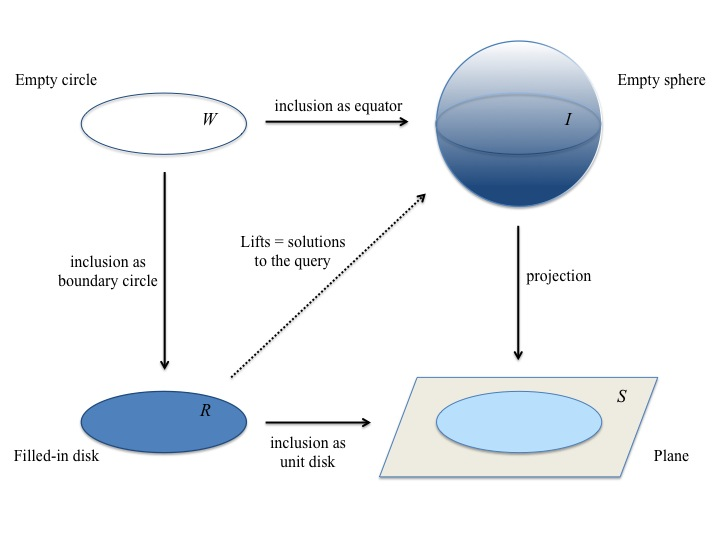
\includegraphics[height=7.5cm]{sphere-topology} 
%}
%
%\ft{Compare}{
%A somewhat contrived analogue: \hspace{.5in}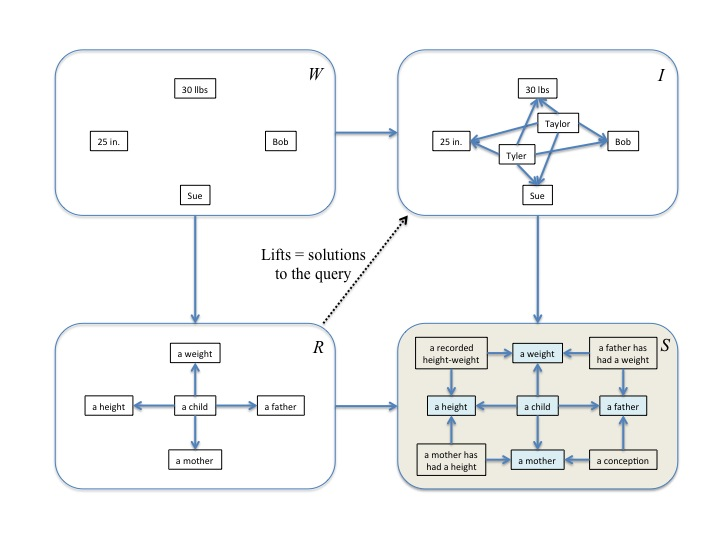
\includegraphics[height=7.5cm]{sphere-database} 
%}
%\fst{Queries as lifting problems}{
%	\sub Given a database instance $I\taking\mcC\to\Set$ with data fibration $\pi\taking I\to\mcC$.
%	\next Queries on $I$ can be written as lifting problems $$\xymatrix{W\ar[r]^p\ar[d]_m&I\ar[d]^\pi\\R\ar[r]_n\ar@{-->}[ur]^\ell&\mcC}$$
%	\next $W$ is the where-clause, $R$ is the result schema.
%	\next We can understand constraints this way too.
%	\endsub
%
%}
%
%\fst{Killer ap?}{
%	\sub We have a tight connection between databases and categories.
%	\next We should be able to import lots of cool mathematics into databases via category theory.
%	\next One example: data mining via algebraic topology.
%	\endsub
%}
%
%\ft{The nerve}{
%	\sub There is a functor $N\taking\Cat\to\Top$. 
%	\next Given a category $\mcC$, its nerve is a topological space $N(\mcC)$. 
%	\next And for any functor $F\taking\mcC\to\mcD$ we get a continuous map $$N(F)\taking N(\mcC)\to N(\mcD).$$
%	\next Topological spaces have many algebraic invariants, such as homology, cohomology, and homotopy groups.
%	\next These give key features of topological spaces. 
%	\next Example: number connected components, number of loops, number of unfilled spheres.
%	\endsub
%}
%
%\ft{The nerve of an instance}{
%	\sub Given a data fibration $\pi\taking I\to\mcC$, we get a continuous map of spaces $N(I)\to N(\mcC)$.
%	\next We can study these spaces and get interesting invariants of the data.
%	\next In fact there is a schema $\mcD$ for which the nerve construction gives an equivalence between $\mcD\set$ and $\Top$!
%	\next So for mathematical schemas, these invariants give just the right answers.
%	\next For the Department store example, we'd see things like which employees are their own manager.
%	\endsub
%}

\section{Conclusion}

\fst{Summary of the talk}{

	\sub I hope the connection between databases and categories is clear.
	\tiny \begin{align*}\parbox{2in}{\begin{tabular}{| l || l | l | l | l |}\hline\multicolumn{5}{| c |}{Employee}\\\hline {\bf Id}&{\bf First}&{\bf Last}&{\bf Mgr}&{\bf Dpt}\\\hline 101&David&Hilbert&103&q10\\\hline 102&Bertrand&Russell&102&x02\\\hline 103&Alan&Turing&103&q10\\\hline\end{tabular}\\\begin{tabular}{| l || l | l |}\hline\multicolumn{3}{| c |}{Department}\\\hline {\bf Id}&{\bf Name}&{\bf Secr}\\\hline q10&Sales&101\\\hline x02&Production&102\\\hline\end{tabular}}&&\mainCatSmall{\mcC=}
\end{align*}\normalsize
	\next I discussed how one can use this connection to facilitate:
		\sub schema mapping and data migration;
		\next formalizing views;
		\next merging database and programming language theory;
		\next merging relational and RDF outlooks;
		\endsub
	\next The main point is that basic category theory provides a self-contained, unified, and profitable approach to databases.
	\endsub
	\begin{center}{\bf Thanks for the invitation to speak!}\end{center}

}


\end{document}

